\documentclass[12pt]{article}
\usepackage{graphicx}
\graphicspath{{./images/}}
\usepackage[a4paper, total={7in, 10in}]{geometry}
\usepackage{xcolor}
\usepackage{wrapfig}
% remember to remove this stuff, this is for dark mode
% \definecolor{mygrey}{rgb}{0.1,0.1,0.1}
% \pagecolor{mygrey}
% \color{white}

\title{Analyzing the effect of the weight of the mass on the distance travelled by a projectile on a trebuchet}
\author{}
\date{Febuary 14th 2024}

\begin{document}

\maketitle

\pagebreak
\tableofcontents

\pagebreak
% ok this is where the background starts
\section{Background}
Often times in the modern world, we may to forefully propell stones, balls, and even people long distances. Historically this was done through the use of catapults, and trebuchets. For example, if Ricko wanted to throw a fairly large rock at James's house, he would have to calculate the weight needed on the end of the trebuchet to launch the projectile with enough energy to make it to Jame's house, and dmaage it.

Now I too sometimes need to launch objects such as balls distances, maybe not at houses, but nonetheless I still need to launch them. So I turned to using a catapult to launch these objects for me, however I did not know how much weight I need to put on the end of the catapult in order to launch the projectile the desired Distance. Thus I decided to investigate the relationship between the distance traveled by the projectile, and the mass on the end of the trebuchet.

This IA mainly focuses on kinematics, as it is measuring the effect of the mass on the end, compared to the distance travelled. Which at the scale the  experiment is being conducted on, would be under kinematics.

The equations, and relationships in question here would be all of the kinematic equations, the equations used to determine force, work, energy, and momentum. These will be used to determine the energy, as well as the relationship between the weight on the end of the trebuchet, and the distance it is flung.

In order to answer this question, a trebuchet will be built, and it will launch a tennis ball, with various weights on the end. The distance travelled will be compared and analysed to determine a relationship between the mass on the end of the trebuchet and the distance travlled by the ball.


\section{Designs and Mechanisms of the trebuchet}

% rewrite this later, this makes no sense LMFAO

The trebuchet that was built for the purposes of this experiment resembles a large lever, with a load on one end (the projectile), and the counter weight on the other. When it comes to force applied to one side is equal to the force on the otherwise multipled by the mechanical advantage. Mechanical advantage can be determined by dividing the (distance from load to fulcrum), by the (distance from effort to fulcrum). Letting \(L\) be the distance from load to fulcrum, letting \(E\) be the distance from effort to fulcrum, and letting the force being experienced by the projectile be represented by \(F\). The equation ends up as;


The first step to determine the speed, and distance the projectile travels is to determine the length which it travels whilst being accelerated. This is a constant length, and is fairly simple to calculate. It is just the arc length. [insert the arc length equation], which results in an arc length of \(174.4 \pm 0.1 \) cm

Then to determine the force, and thus acceleration, the \(F_{net}\) must be found, which is the sum of all the forces acting on the ball. In addition mechanical advantage must be taken into consideration. This results in the equation \(F_{net} = \frac{76.2}{124.46} \cdot 9.81 \cdot M_{cw} - 9.81 \cdot M_{t}\) being the counter weight's mass, and \(M_{t}\) being the tennis ball's weight. In addition the counterweight's force is multiplied by \(\frac{76.2}{124.46}\) as that is the value for mechanical advantage. Then to find the acceleration of the projectile, simply divide the \(F_{net}\) by the mass of the object, \( \frac{0.612 \cdot 9.81 \cdot M_{cw} - 9.81 \cdot M_{t}}{M_{t}} = a_{t}\)

Now we can use the equation \(v^{2} = 2 \cdot a_{t} \cdot s\), replacing everything, we can see the equation like, the 1.744 represents the length of the arc
\[ v = \sqrt{2 \cdot  \frac{0.612 \cdot 9.81 \cdot M_{cw} - 9.81 \cdot M_{t}}{M_{t}} \cdot 1.744} m/s\]
\section{Hypothesis}
From the equation above, it can be theorised that; If the mass of the counterweight increases, the distance travelled will increase porportinal to that equation

\section{Variables}
\subsection{Controlled variables}
\begin{center}
\begin{tabular}{||c c||}
 \hline
 Variable & Reason for being Controlled  \\ [0.5ex]
 \hline\hline
 Launch Angle & 6  \\
 \hline
 Projectile Size & a \\
 \hline
 Projectile Weight & g \\
 \hline
 Projectile Shape & h \\
 \hline
  Trebuchet mechanism & a \\
 \hline
  Shape of projectile & a \\
  \hline
  Shape of Counterweight & y \\
  \hline
\end{tabular}
\end{center}

\subsection{Dependent variable}
T
\subsection{Independent variable}

\paragraph{finding velocity}
\begin{wrapfigure}{r}{0.5\textwidth} %this figure will be at the right
  \centering
  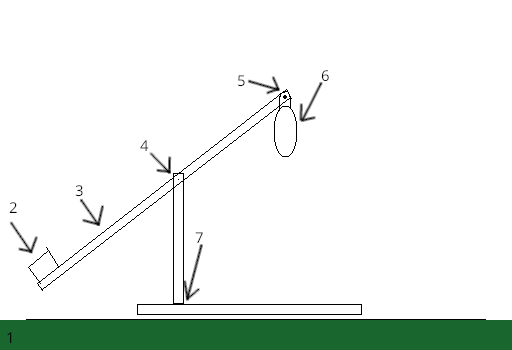
\includegraphics[width=0.5\textwidth]{cataaa}
\end{wrapfigure}


\end{document}
